%license:BSD-3-Clause
%copyright-holders:Michele Maione
%============================================================
%
%	Piattaforma di cloud gaming per giochi arcade
%
%============================================================
\chapter{Tecnologie}

In questo capitolo 

\section{Sistema proposto}
Le caratteristiche principali del progetto, che sono state vincolanti nella scelta delle tecnologie da utilizzare, sono la portabilità e la possibilità di utilizzare il sistema senza dover installare software aggiuntivi, e per questi vincoli lato client la scelta è ricaduta sul browser web. Le tecnologie di streaming per i browser web ad oggi sono: WebSocket, HLS, DASH e WebRTC\cite{Audio_and_video_delivery}.

WebSocket è un protocollo di comunicazione che fornisce un canale full-duplex su una singola connessione TCP, con una latenza inferiore rispetto ad HLS e DASH.

HTTP Live Streaming (HLS) è il protocollo di streaming ad alta latenza più popolare su protocollo HTTP per video on demand (video preregistrato) sviluppato da Apple.

Dynamic Adaptive Streaming over HTTP (DASH) è una tecnica di streaming con bit-rate adattivo del Moving Picture Experts Group (MPEG), che consente lo streaming di alta qualità di contenuti multimediali su protocollo HTTP.

Web Real-Time Communication (WebRTC) è un progetto per la comunicazione in tempo reale basato sul protocollo RTP (Real-time Transport Protocol)\cite{High_Performance_Browser_Networking}.

\begin{figure}[H]
	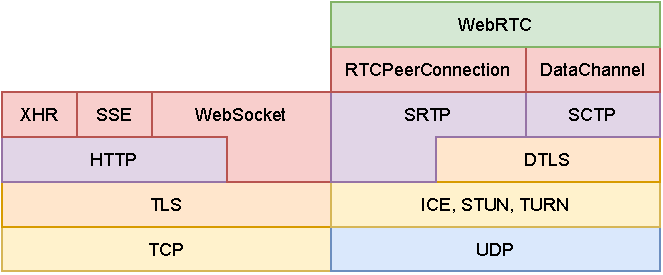
\includegraphics[width=\linewidth]{immagini/webprotocols}
	\caption{API, protocolli e servizi di rete del browser di alto livello}
	\label{fig:webprotocols}
\end{figure}

L'esigenza per la quale nasce questo progetto è far conoscere alle nuove generazioni i videogiochi che hanno fatto la storia e dare la possibilità di poter giocare ancora a macchine che ormai hanno cessato di funzionare per motivi di obsolescenza, e proprio per questo la progettazione si è basata, sì sullo streaming via rete, ma con un'ottica incentrata sull'utilizzo in stand di retro-gaming in eventi relativi all'informatica e ai videogiochi, quindi sulla rete locale dell'evento con gli utenti connessi tramite WiFi. In quest'ottica la differenza di velocità tra TCP e RTP è trascurabile, e la scelta è ricaduta su WebSocket perché è un protocollo di comunicazione standardizzato dal 2011, è pienamente supportato da tutti i browser moderni, è semplice e non richiede l'utilizzo di protocolli aggiuntivi o configurazioni complesse a differenza di WebRTC.

\begin{figure}[H]
	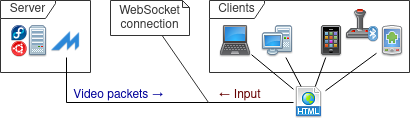
\includegraphics[width=\linewidth]{immagini/proposed_system}
	\caption{Panoramica del sistema}
	\label{fig:proposed_system}
\end{figure}

Come mostrato in Fig. \ref{fig:proposed_system} il sistema è costituito dal server di gioco, che può essere Linux, Windows o macOS, su cui è in esecuzione la versione modificata di MAME, e una pagina HTML5 che funge da front-end. Il programma è in ascolto per connessioni WebSocket con parametri (per es.: il nome del gioco, l'ID del player, l'ID della partita). Una volta stabilita la connessione, il server invia informazioni sulla dimensione e le proporzioni del video e avvia il gioco. Il rendering e il missaggio audio del gioco vengono generati tramite SDL\footnote{SDL: Simple DirectMedia Layer, una libreria multipiattaforma ed open-soure per il multimedia}, codificati e pacchettizzati in MPEG-TS\footnote{MPEG-TS: MPEG transport stream, è un contenitore digitale per la trasmissione e l'archiviazione audio-video.} tramite FFmpeg\footnote{FFmpeg è una suite open-source di librerie e programmi per la gestione di video, audio, e altri file multimediali e stream.}. I pacchetti vengono inviati tramite WebSocket al client.

Lato client vari script si occupano di decodificare i dati audio-video ricevuti, catturare e inviare l'input dell'utente, sia dalla tastiera che dal gamepad, al server tramite WebSocket.

\section{MPEG}
Lorem ipsum dolor sit amet, consectetur adipiscing elit, sed do eiusmod tempor incididunt ut labore et dolore magna aliqua. Ut enim ad minim veniam, quis nostrud exercitation ullamco laboris nisi ut aliquip ex ea commodo consequat. Duis aute irure dolor in reprehenderit in voluptate velit esse cillum dolore eu fugiat nulla pariatur. Excepteur sint occaecat cupidatat non proident, sunt in culpa qui officia deserunt mollit anim id est laborum.

\subsection{Compression}
Lorem ipsum dolor sit amet, consectetur adipiscing elit, sed do eiusmod tempor incididunt ut labore et dolore magna aliqua. Ut enim ad minim veniam, quis nostrud exercitation ullamco laboris nisi ut aliquip ex ea commodo consequat. Duis aute irure dolor in reprehenderit in voluptate velit esse cillum dolore eu fugiat nulla pariatur. Excepteur sint occaecat cupidatat non proident, sunt in culpa qui officia deserunt mollit anim id est laborum.

\subsection{Video}
Lorem ipsum dolor sit amet, consectetur adipiscing elit, sed do eiusmod tempor incididunt ut labore et dolore magna aliqua. Ut enim ad minim veniam, quis nostrud exercitation ullamco laboris nisi ut aliquip ex ea commodo consequat. Duis aute irure dolor in reprehenderit in voluptate velit esse cillum dolore eu fugiat nulla pariatur. Excepteur sint occaecat cupidatat non proident, sunt in culpa qui officia deserunt mollit anim id est laborum.

\subsection{Audio}
Lorem ipsum dolor sit amet, consectetur adipiscing elit, sed do eiusmod tempor incididunt ut labore et dolore magna aliqua. Ut enim ad minim veniam, quis nostrud exercitation ullamco laboris nisi ut aliquip ex ea commodo consequat. Duis aute irure dolor in reprehenderit in voluptate velit esse cillum dolore eu fugiat nulla pariatur. Excepteur sint occaecat cupidatat non proident, sunt in culpa qui officia deserunt mollit anim id est laborum.

\subsection{Trasmission}
Lorem ipsum dolor sit amet, consectetur adipiscing elit, sed do eiusmod tempor incididunt ut labore et dolore magna aliqua. Ut enim ad minim veniam, quis nostrud exercitation ullamco laboris nisi ut aliquip ex ea commodo consequat. Duis aute irure dolor in reprehenderit in voluptate velit esse cillum dolore eu fugiat nulla pariatur. Excepteur sint occaecat cupidatat non proident, sunt in culpa qui officia deserunt mollit anim id est laborum.



\section{FFmpeg}
Lorem ipsum dolor sit amet, consectetur adipiscing elit, sed do eiusmod tempor incididunt ut labore et dolore magna aliqua. Ut enim ad minim veniam, quis nostrud exercitation ullamco laboris nisi ut aliquip ex ea commodo consequat. Duis aute irure dolor in reprehenderit in voluptate velit esse cillum dolore eu fugiat nulla pariatur. Excepteur sint occaecat cupidatat non proident, sunt in culpa qui officia deserunt mollit anim id est laborum\cite{FFmpeg_Documentation}.

\subsection{Libs.}
Lorem ipsum dolor sit amet, consectetur adipiscing elit, sed do eiusmod tempor incididunt ut labore et dolore magna aliqua. Ut enim ad minim veniam, quis nostrud exercitation ullamco laboris nisi ut aliquip ex ea commodo consequat. Duis aute irure dolor in reprehenderit in voluptate velit esse cillum dolore eu fugiat nulla pariatur. Excepteur sint occaecat cupidatat non proident, sunt in culpa qui officia deserunt mollit anim id est laborum.



\section{Simple DirectMedia Layer (SDL)}
SDL è una libreria che fornisce accesso di basso livello ad audio, tastiera, mouse, gamepad, hardware 3D e framebuffer 2D su più piattaforme, anche mobili. SDL è costruito sopra le API di visualizzazione video di O.S., una libreria di rendering 3D e una libreria che si interfaccia alla scheda audio\cite{SDL_Wiki}.

\begin{figure}[H]
	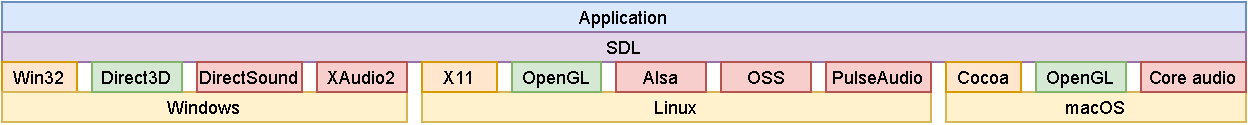
\includegraphics[width=\linewidth]{immagini/sdl}
	\caption{Livelli di astrazione di diverse piattaforme SDL}
	\label{fig:sdl}
\end{figure}

\subsection{Video}
Il MAME è in grado di emulare giochi 3D ma poiché si sta emulando un monitor fisico, ciò che viene inviato alle varie librerie grafiche è un insieme di primitive e texture da disegnare, e per questo motivo il disegno viene sempre eseguito in 2D.

\begin{figure}[H]
	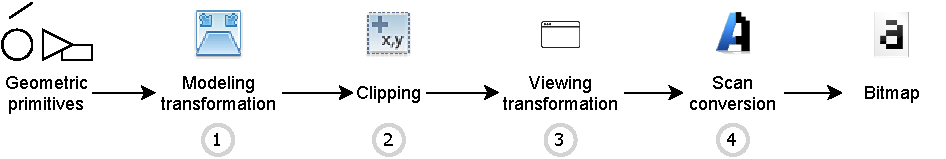
\includegraphics[width=\linewidth]{immagini/rendering_pipeline}
	\caption{Pipeline di rendering 2D}
	\label{fig:rendering_pipeline}
\end{figure}

Quando la finestra viene inizializzata, viene creato un contesto di rendering 2D SDL per la finestra tramite la funzione \textit{CreateRenderer}. Per ogni frame di macchina emulato c'è una fase di disegno usando \textit{SetRenderDrawColor}, \textit{RenderFillRect} e \textit{RenderDrawLine}. Alla fine la funzione \textit{RenderPresent} viene utilizzato per mostrare la cornice sulla finestra.

Nella sezione \ref{SDL_renderer} vengono introdotte altre funzioni, usate per modificare questo comportamento standard descritto sopra.


\subsection{Audio}
Lorem ipsum dolor sit amet, consectetur adipiscing elit, sed do eiusmod tempor incididunt ut labore et dolore magna aliqua. Ut enim ad minim veniam, quis nostrud exercitation ullamco laboris nisi ut aliquip ex ea commodo consequat. Duis aute irure dolor in reprehenderit in voluptate velit esse cillum dolore eu fugiat nulla pariatur. Excepteur sint occaecat cupidatat non proident, sunt in culpa qui officia deserunt mollit anim id est laborum.



\section{Web APIs}
Le API Web sono un insieme di API e interfacce che comprendono la potente capacità di creazione di script del Web. A seguire quelli utilizzati in questo progetto\cite{Web_APIs}.

\subsection{WebSocket}
WebSocket è un protocollo di comunicazione del computer che fornisce canali di comunicazione full-duplex su una singola connessione TCP. È compatibile con HTTP perché l'handshake WebSocket utilizza l'intestazione di aggiornamento HTTP per passare dal protocollo HTTP al protocollo WebSocket. È supportato nativamente da tutti i browser e il suo utilizzo è simile ai normali socket sia sul lato client che su quello server. Per questi motivi è il protocollo di comunicazione generico più utilizzato sul web\cite{WebSocket_Web_APIs}.

\subsection{Canvas API}
L'API Canvas fornisce un mezzo per disegnare grafica tramite JavaScript, si concentra principalmente sulla grafica 2D ma quando viene utilizzata dall'API WebGL può disegnare grafica 2D e 3D con accelerazione hardware. È completamente supportato da tutti i browser\cite{Canvas_API}.

\subsection{WebGL API}
WebGL è un'API JavaScript, progettata e gestita dal gruppo no-profit Khronos, per il rendering di grafica 2D e 3D interattiva che consente l'utilizzo accelerato dalla GPU della fisica e dell'elaborazione e degli effetti delle immagini. WebGL 1.0 è supportato su tutti i browser, mentre WebGL 2.0 viene testato su Safari\cite{WebGL}.



\section{JavaScript libraries}
Per il front-end, sono state utilizzate librerie JavaScript open source per la gestione degli input e per la decodifica del filmato.

\subsection{JSMpeg}
JSMpeg è una libreria JavaScript composta da un demuxer MPEG-TS, video MPEG1 e decoder audio MP2, renderer WebGL e Canvas2D e output audio WebAudio. JSMpeg può caricare video statici tramite Ajax e consente lo streaming a bassa latenza ($\sim$50ms) tramite WebSocket, è rilasciato con licenza MIT\cite{JSMpeg}.

\subsection{Keypress}
Keypress è un'utilità JavaScript che cattura l'input da tastiera focalizzata sull'input per i giochi, rilasciata con la licenza Apache 2.0. Viene utilizzato per gestire l'input da tastiera nel front-end\cite{Keypress}.

\subsection{GameController.js}
GameController.js è una libreria che utilizza JavaScript e l'API Gamepad standard, è rilasciata con licenza MIT. Nel front-end viene utilizzato per gestire i gamepad, per consentire il multiplayer da divano\cite{gameController_js}.